% !TeX root = ../main.tex
\section{Experiments}

\subsection{Datasets and Protocols}
In this work, we measure the model performance on the Tripitaka Koreana in Han (TKH) Dataset and the Multiple Tripitaka in Han (MTH) Dataset~\cite{tkhmth}. Following~\cite{jla},
we use the combined version of TKH and MTH2200, which is named MTHv2. Specifically, the MTHv2 dataset provides line-level annotation, character-level annotation, and ``boundary lines'' which include reading order information. In this work, we mainly use the line-level annotation which takes the minimum cost to obtain. 

Protocol-wise, we mainly evaluate the overall performance of our method on the full testing set, following the exact split from ~\cite{jla}, which randomly split the MTHv2 dataset into the training set and the testing set with the ratio of 3:1. It is important to note that our training and test sets are kept completely consistent with ~\cite{jla}. We did not use any additional data such as synthetic data or pre-trained models.


Besides the benchmarking, we conduct extensive ablative and behavior analysis to validate the proposed approach.


\subsection{Implementation details}
The code is implemented based on the OpenCCD code base~\cite{vsdf}. The input image is resized to $32$ pixels by width and center padded to $32\times 320$ image. The model is trained for $\SNepoches$ epochs with batch size set to $64$ from scratch. % If you want to introduce the learning rate etc go ahead.

The experiments are conducted on a virtual machine with Pytorch-$1.12.1$, TorchVision-$0.13.1$ CUDA-$11.2$, and Ubuntu $22.04$. Training from scratch using an Nvidia RTX 4090 GPU would typically take around 10 hours to complete 128 epochs. Depending on the model, when the batch size is set to $64$, the GPU memory usage is about 11-21GB.

% The models, codes, and documents are released on~\url{xxx}

\subsection{Comparison with SOTA}
\begin{table}[]
    \centering
    \caption{Comparison to State of The Art methods on the MTHv2~\cite{jla} dataset. LA refers to Line Accuracy.}

    \begin{tabular}{c|c|ccc}
        \hline
         Name & Venue & AR & \textbf{CR} & LA \\
         \hline
         JLA~\cite{jla}& icfhr' 20&94.08 & 95.09 & -\\
         \hline
         VSDF*\cite{vsdf}& CVPR' 22 &93.14 &94.41 &67.59 \\
         \hline
         Ours&- &\textbf{94.21} & \textbf{95.27} & \textbf{70.77} \\
        \hline
    \end{tabular}
    \label{tab:my_label}
\end{table}

\subsection{Ablative Studies}
We first conduct module-level ablative experiments to validate the effectiveness of the proposed spindle network. Then, we provide an extended architecture-level ablative analysis, discussing various other possible designs and why they are less feasible than the proposed spindle-shaped network.  

\subsubsection{Module-level Ablative}


\begin{figure}[!t]
    \begin{center}
    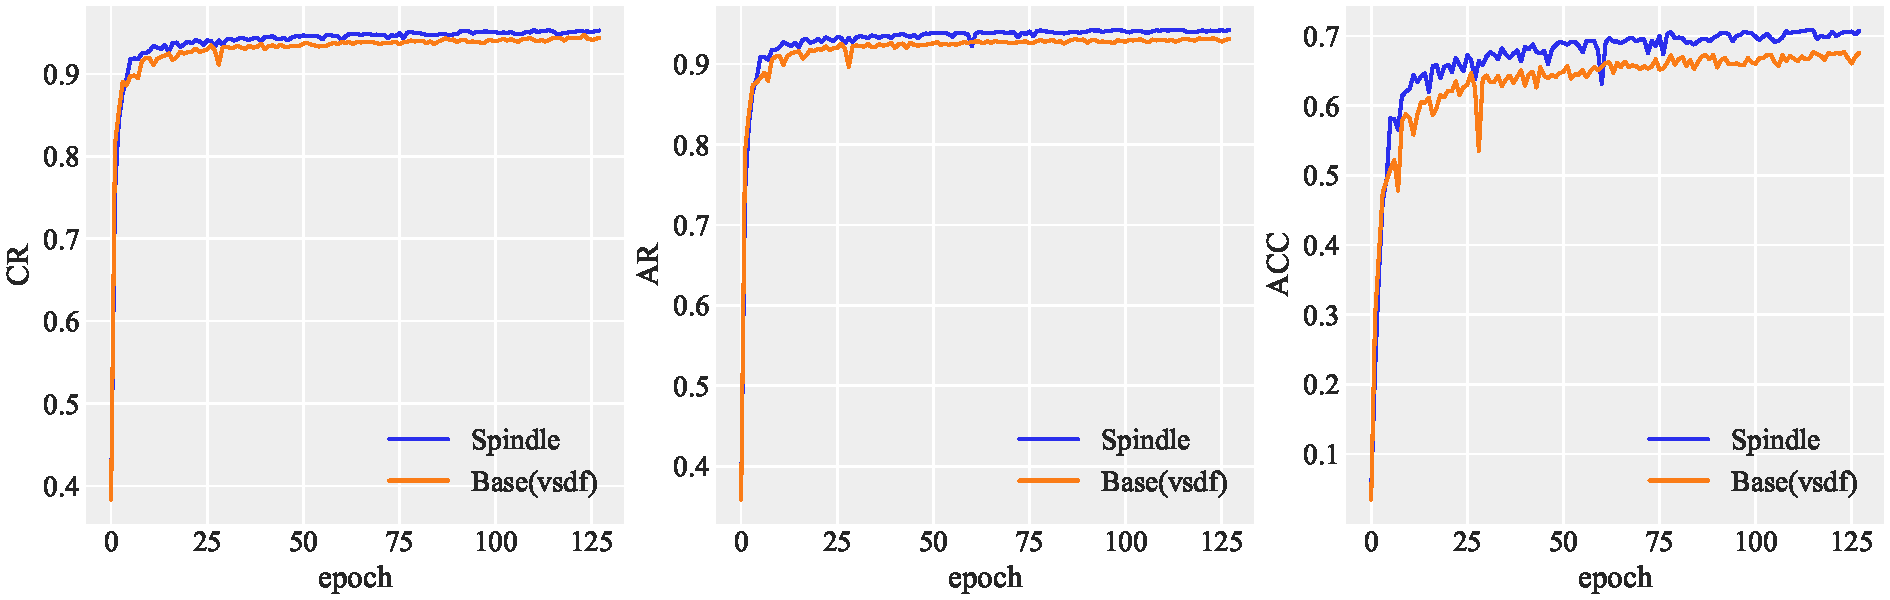
\includegraphics[width=1.0\linewidth]{figures/quantitative.pdf}
    \end{center}
    \caption{quantitative results}
    \label{fig:quantitative}
\end{figure}

    

In this part, we perform ablative studies on the design of the spindle network, the quantitative results are shown in Fig.~\ref{fig:quantitative}.% insert your analysis here


\begin{figure}[!t]
    \begin{center}
    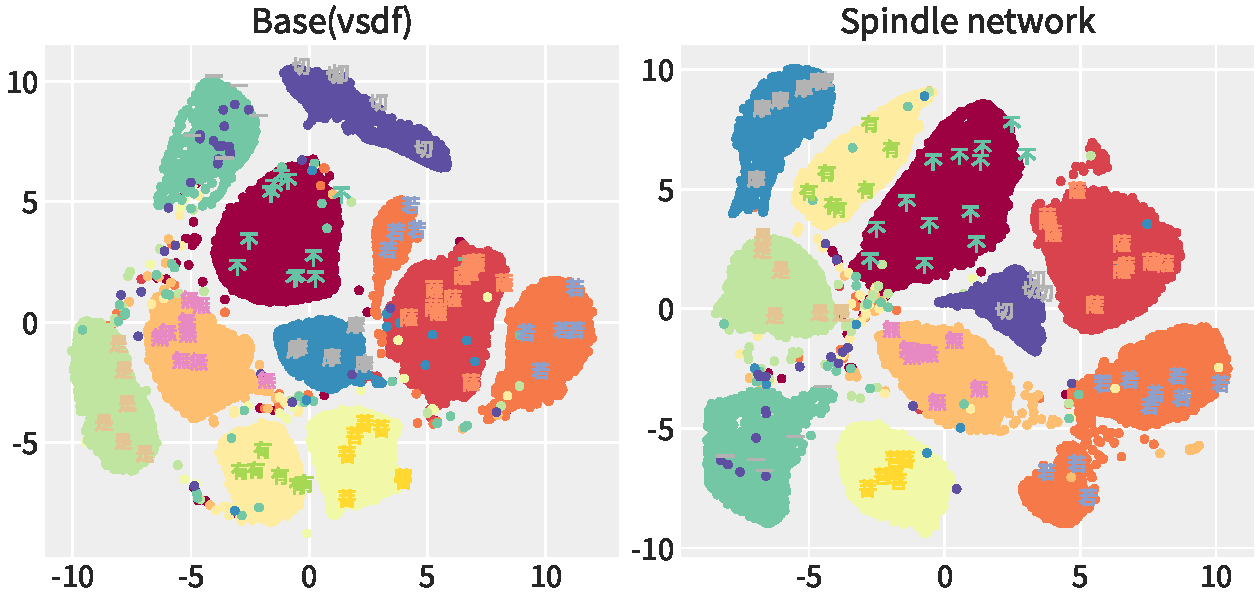
\includegraphics[width=1.0\linewidth]{figures/tsne.pdf}
    \end{center}
    \caption{Visualization of TSNE features from the top 10 frequencies.}
    \label{fig:tsne}
\end{figure}

    
We further perform qualitative analysis to find out how the spindle net affects the character features, shown in Fig.~\ref{fig:tsne}  



\subsubsection{Architecture-level Ablative}
In this section, we first demonstrate how the spindle-ness affects the performance. Then we discuss the structural sensitivity, i. e. which convolution layer deserves the most parameters.

We first define the term ``spindle-ness'' by the largest channel number, % please change this one. 
and then perform quantitative analysis on the relation between the ``spindle-ness'' and the model performance.
The results are shown in Fig~\ref{fig:spindleness}, ... % insert your analysis here.

\begin{figure}[!t]
	\centering
	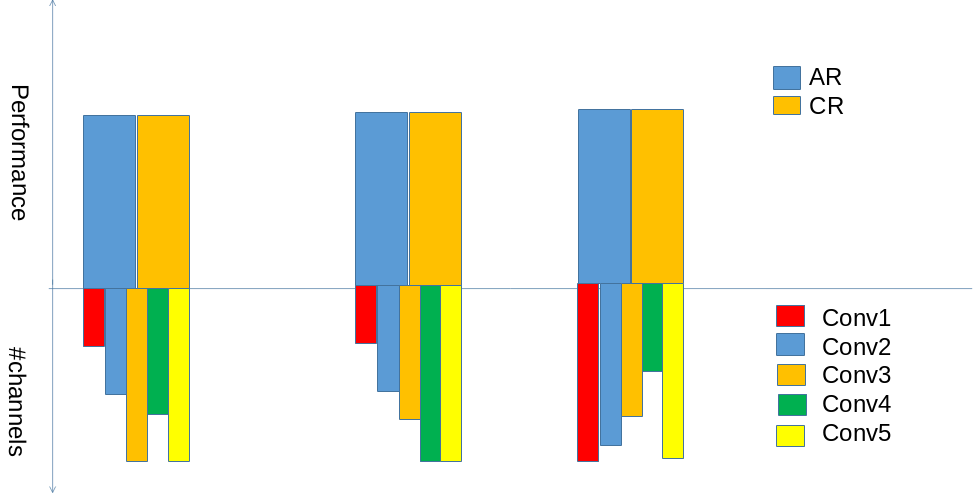
\includegraphics[width=\linewidth]{figures/archabl.png}
	\caption
    {The ablative on architecture. Note we kept the channel number of the output layer (conv5) fixed to rule out affects from other module to the performance.}
	\label{fig:archabl}
\end{figure}
We then analyze the structural sensitivity, i.e., which layer needs the most parameters. The results are shown in Fig.~\ref{fig:archabl}. ... % insert your analysis here.

\subsection{Behaviour Analysis}

In this part, we break down the results into classes to see which classes are more affected by the spindle network and why. 
\subsubsection{Per-class Performance Analysis}


\begin{figure}[!t]
    \begin{center}
    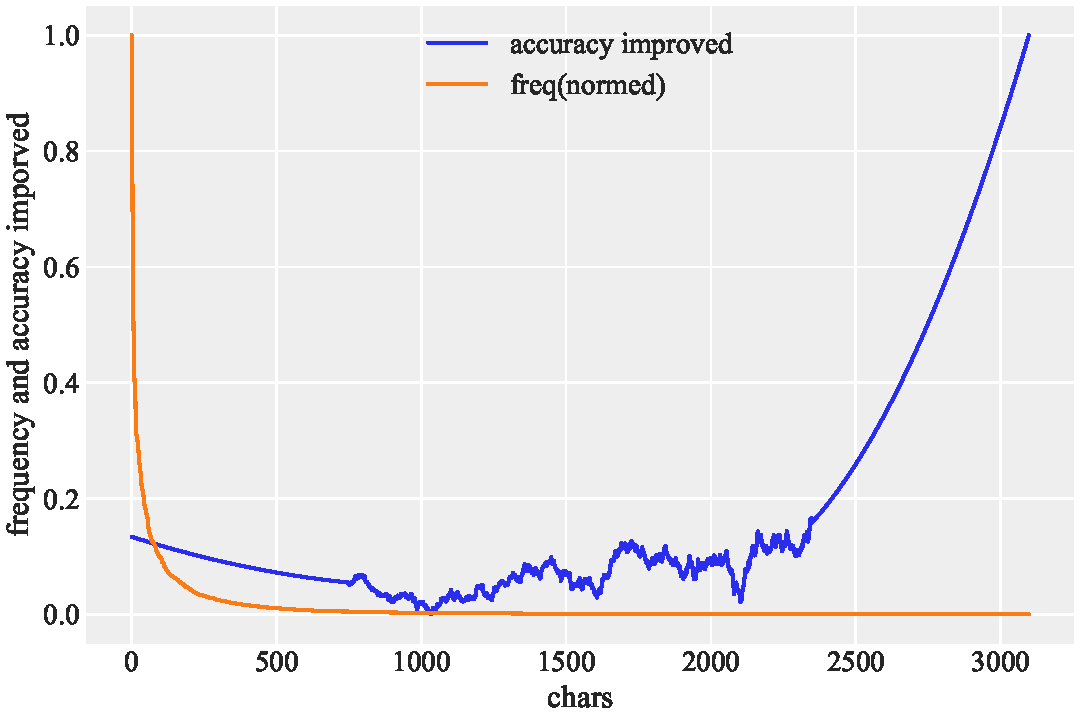
\includegraphics[width=1.0\linewidth]{figures/freqvsimprovement.pdf}
    \end{center}
    \caption{frequency and accuracy imporved}
    \label{fig:freqvsimprovement}
\end{figure}

    
This provides per-class performance change analysis to provide more insight on the improving pattern. 
The overall trend is shown in ~\ref{fig:freqvsimprovement}. 
% You claimed it would improve tail classes, now prove it. 

%Also try to give a description of the behavior of the head classes, try to give a few assumptions, and leave the proof as homework to the readers.


\subsubsection{Zero-shot Performance on MTHv2}
This section discusses the zero-shot capability of the proposed model. Specifically, we report the performances of samples that contain unseen characters to give an estimation of how well the proposed modules handle the unseen characters. In the base model, the accuracy of new characters is \textbf{52.72}, while in the spindle network, the accuracy of new characters is \textbf{53.97}.


